\documentclass{article}
\usepackage{fullpage}
\usepackage{amsmath}
\usepackage{amsfonts}
\usepackage{tipa}
\usepackage{tikz}
\usetikzlibrary{arrows, automata, matrix}
\begin{document}
\begin{center}
\Large{Finite State Acceptor for Nanjing Dialect Tone Sandhi}
\end{center}
\vspace{1cm}
First, I will define the alphabet and introduce the prohibited 2-factors:
\par
\vspace{.5cm}
$\Sigma$ = \{a, b, c, d, e\}
\hspace{2cm}
\begin{tabular}{ccl}
a	&	=	&	HL	\\
b	&	=	&	LH	\\
c	&	=	&	H	\\	
d	&	=	&	L	\\
e	&	=	&	H\textipa{P}	\\
\end{tabular}
\hspace{2cm}
$\overline{F_2}$ = \{aa, be, ce, da, dd, de\}
\newline
\newline
\newline
\newline
The following FSA accepts well-formed strings in the language:
\vspace{1cm}
\begin{center}
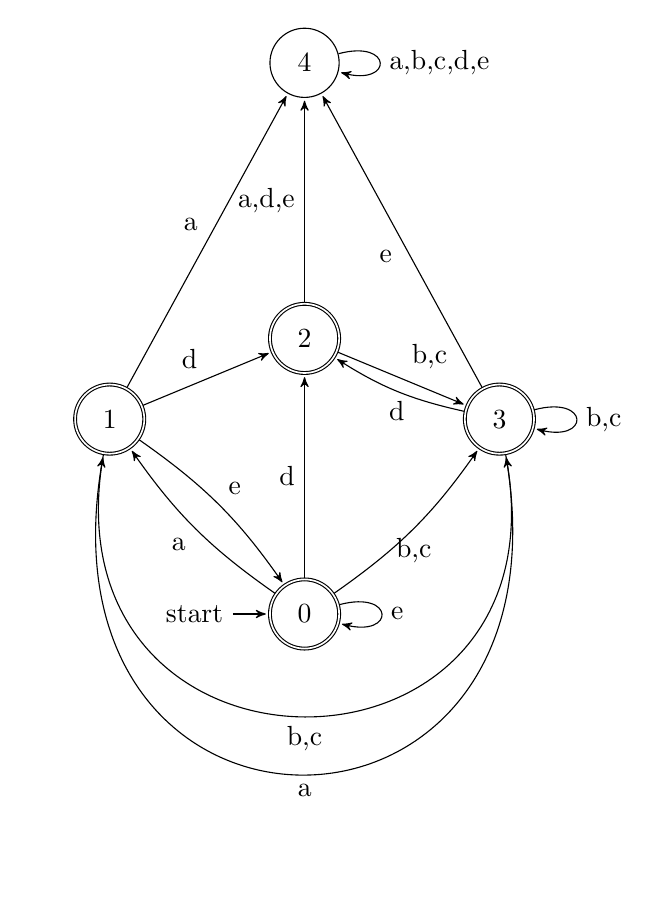
\begin{tikzpicture}[->,>=stealth',shorten >=1pt,auto, node distance=3.5cm]

  \node[state, initial, accepting]  		(0)                               		{$0$};
  \node[state, accepting]          	(1)  	[above left of=0]		{$1$};
  \node[state, accepting]    	(2)     [above of=0] 	{$2$};
  \node[state, accepting]	  	(3)    	[above right of=0] 	{$3$};
  \node[state]			(4)	[above of=2]		{$4$};
 
  
\path[->]
(0)	edge [bend left=10] node {a} (1)
	edge node {d} (2)
	edge [bend right=10, below] node {b,c} (3)
	edge [loop right] node {e} (0)	
(1)	edge [bend left=10] node {e} (0)
	edge node {a} (4)
	edge node {d} (2)
	edge [bend right=100,below,distance=4.5cm] node {b,c} (3)
(2)	edge node {b,c} (3)
	edge node {a,d,e} (4)
(4)	edge [loop right] node {a,b,c,d,e} (4)
(3)	edge node {e} (4)
	edge [bend left=10, below] node {d} (2)
	edge [bend left=100,below,distance=5.5cm] node {a} (1)
	edge [loop right] node {b,c} (3);
	
\end{tikzpicture}
\end{center}
\vspace{.5cm}
This FSA is a tuple ($Q, \Sigma, q_0, F, \delta$) where
\begin{center}
\begin{tabular}{rcl}
$Q$			&	=	&	\{0, 1, 2, 3, 4\}	\\
$\Sigma$		&	=	&	\{a, b, c, d, e\}	\\
$q_0$			& 	$\in$	&	$Q$			\\
$F \subseteq Q$	&	=	&	\{0, 1, 2, 3\}		\\
domain of $\delta$&	=	&	$Q \times \Sigma$		\\
\end{tabular}
\end{center}
\pagebreak{}
\begin{center}
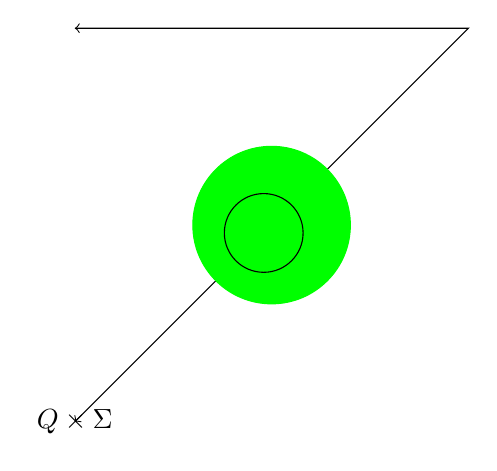
\begin{tikzpicture}
	\draw [<->] (0,0) -- (5,5) -- (0,5);
	\draw [fill, color = green](2.5, 2.5) circle [radius =1];
	\draw (2.4, 2.4) circle [radius = .5];
	\node at (0,0) {$Q \times \Sigma$};
	%\draw (5,0) -- (0,5);
	%\draw (0,0) -- (0,5);
	%\draw (5,0) -- (5,5);
\end{tikzpicture}
\end{center}
\medskip{}
\begin{center}
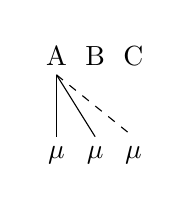
\begin{tikzpicture}
	\matrix [row sep=.8cm] {
	\node(a){A}; & \node(b){B}; & \node(c){C}; \\
	\node(m1){$\mu$}; & \node(m2){$\mu$}; & \node(m3){$\mu$}; \\
	};
	\draw (a) -- (m1);
	\draw (a.south) -- (m2.north);
	\draw [dashed] (a.south) -- (m3.north);
\end{tikzpicture}
\end{center}
\bigskip{}
\begin{center}
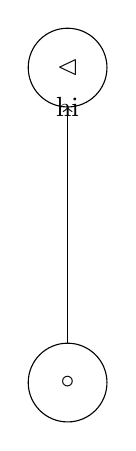
\begin{tikzpicture}
	\draw (0, 0) circle [radius = .5] node {$\circ$};
	\draw (0, 4) circle [radius = .5] node {$\lhd$};
	\draw [->] (0, .5) -- (0, 3.5) node {hi};
\end{tikzpicture}
\end{center}
\begin{center}
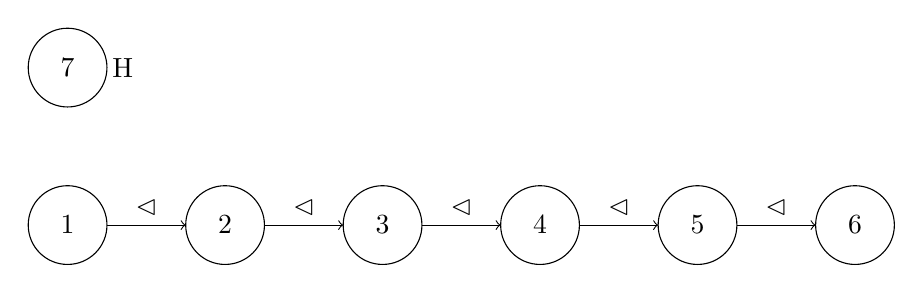
\begin{tikzpicture}
	\draw (-5,2) circle [radius = .5] node {$7$} node at (-4.3,2) {H};
	\draw (-5, 0) circle [radius = .5] node {$1$};
	\draw (-3, 0) circle [radius = .5] node {$2$};
	\draw (-1, 0) circle [radius = .5] node {$3$};
	\draw (1, 0) circle [radius = .5] node {$4$};
	\draw (3, 0) circle [radius = .5] node {$5$};
	\draw (5, 0) circle [radius = .5] node {$6$};
	\draw [->] (-4.5,0) -- (-3.5,0) node [above, pos=.5] {$\lhd$};
	\draw [->] (-2.5,0) -- (-1.5,0) node [above, pos=.5] {$\lhd$};
	\draw [->] (-.5,0) -- (.5,0) node [above, pos=.5] {$\lhd$};
	\draw [->] (1.5,0) -- (2.5,0) node [above, pos=.5] {$\lhd$};
	\draw [->] (3.5,0) -- (4.5,0) node [above, pos=.5] {$\lhd$};
\end{tikzpicture}
\end{center}
\vspace{.3cm}
\begin{center}
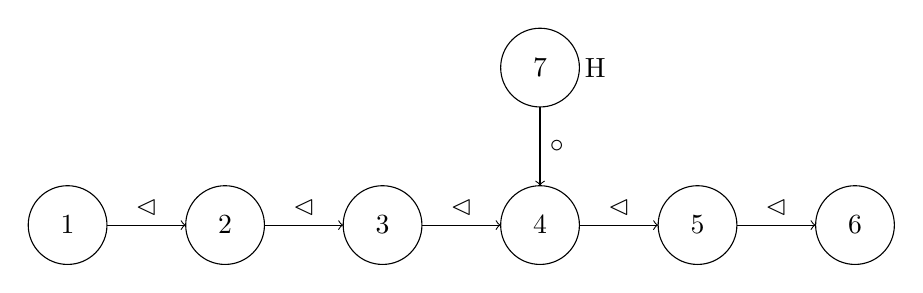
\begin{tikzpicture}
	\draw (1,2) circle [radius = .5] node {$7$} node at (1.7,2) {H};
	\draw (-5, 0) circle [radius = .5] node {$1$};
	\draw (-3, 0) circle [radius = .5] node {$2$};
	\draw (-1, 0) circle [radius = .5] node {$3$};
	\draw (1, 0) circle [radius = .5] node {$4$};
	\draw (3, 0) circle [radius = .5] node {$5$};
	\draw (5, 0) circle [radius = .5] node {$6$};
	\draw [->] (-4.5,0) -- (-3.5,0) node [above, pos=.5] {$\lhd$};
	\draw [->] (-2.5,0) -- (-1.5,0) node [above, pos=.5] {$\lhd$};
	\draw [->] (-.5,0) -- (.5,0) node [above, pos=.5] {$\lhd$};
	\draw [->] (1.5,0) -- (2.5,0) node [above, pos=.5] {$\lhd$};
	\draw [->] (3.5,0) -- (4.5,0) node [above, pos=.5] {$\lhd$};
	\draw [->] (1,1.5) -- (1,.5) node [right, pos=.5] {$\circ$};
\end{tikzpicture}
\end{center}

\end{document}